\documentclass[conference]{IEEEtran}
\IEEEoverridecommandlockouts

\usepackage{cite}
\usepackage{amsmath,amssymb,amsfonts}
\usepackage{graphicx}
\usepackage{textcomp}
\usepackage{xcolor}
\usepackage{booktabs}
\usepackage{url}
\graphicspath{{figures/}}
\usepackage[hidelinks]{hyperref}

\begin{document}

\title{Dominance Redefined: Visualizing Max Verstappen's 2023 Formula 1 Season}

\author{\IEEEauthorblockN{Varun Brahma}
\IEEEauthorblockA{Department of Computer Science\\
University of San Francisco\\
San Francisco, CA, USA\\
Email: \texttt{vbrahma@dons.usfca.edu}}
}

\maketitle

\begin{abstract}
Max Verstappen's 2023 Formula 1 season is often summarized through headline records such as 19 wins and 575 points, but raw totals alone do not explain how dominance developed, how much of it can be attributed to the car, or how the season compares with other elite performances. This project presents an interactive visualization system that examines the season at four levels: race-by-race championship progression, comparison with teammate Sergio P\'erez, comparison with historically dominant Formula 1 seasons, and comparison with peak athletes from other sports. The visualizations combine animated standings, small multiples, normalized parallel coordinates, and empirical cumulative distribution functions to move from familiar race statistics toward more careful cross-era and cross-sport comparisons. The project shows that Verstappen's dominance emerged through sustained mid-season separation, exceeded his teammate's results despite identical machinery, ranked among the strongest Formula 1 seasons ever, and remained comparable with elite seasons in other sports when performance was translated to a shared percentile scale. The report also discusses the limits of normalization, the design choices behind each view, and the tradeoffs involved in comparing unlike competitive environments.
\end{abstract}

\begin{IEEEkeywords}
information visualization, sports analytics, Formula 1, D3.js, small multiples, parallel coordinates, empirical cumulative distribution function
\end{IEEEkeywords}

\section{Introduction}
Max Verstappen's 2023 Formula 1 season is remembered as dominant, but that description is more interesting when it becomes measurable. Formula 1 naturally supports visual analysis through race-by-race progression, cumulative point accumulation, finishing consistency, and qualifying-versus-race outcomes; Verstappen's season is especially suitable because it exposes not only frequent victories, but also how competitive separation widened over time. A final points total reveals the endpoint of a season without showing how the gap formed; a constructor advantage can obscure the driver's contribution; and raw records from different eras become difficult to compare when scoring systems and season lengths change. This project therefore asks a more precise question: \emph{what does dominance look like when it is examined over time, against the closest available control, across Formula 1 history, and against elite seasons in other sports?}

The system is designed for readers who understand basic computing concepts but are not visualization specialists. Rather than relying on one summary chart, it uses coordinated narrative sections that progressively widen the lens from the 2023 championship to historical and cross-sport comparison. This structure follows established visualization principles: overview before detail, comparison through aligned views, and careful transformation of data when direct comparison would be misleading \cite{munzner2014visualization,wilke2019fundamentals,segel2010narrative}.

The project objectives are:
\begin{itemize}
    \item Show how Verstappen's lead developed across the 22-race 2023 season.
    \item Separate driver performance from car performance by comparing Verstappen with teammate Sergio P\'erez in the same Red Bull RB19.
    \item Compare Verstappen's 2023 season with historically dominant Formula 1 seasons using normalized rate metrics.
    \item Compare sustained dominance across sports without treating unlike raw statistics as directly equivalent.
\end{itemize}

\section{Related Work}
This project draws first from the course's core visualization texts. Munzner's task-centered framing informed the decision to choose a different chart for each analytical question instead of forcing one visual form to answer everything \cite{munzner2014visualization}. Wilke's discussion of small multiples and honest comparison shaped the teammate view, where repeated aligned panels make differences legible without overplotting \cite{wilke2019fundamentals,tufte1983visual,cleveland1984graphical}. Segel and Heer's narrative-visualization framework, along with related work on visualization rhetoric, is especially relevant because the final site is neither a static dashboard nor a fully author-controlled slideshow: it uses a guided sequence of sections while still allowing reader-driven exploration inside each view \cite{segel2010narrative,hullman2011visualization,shneiderman1996eyes}.

Sports visualization literature argues that athletics data is particularly rich because it combines temporal, comparative, and narrative questions, making it a fertile setting for interactive analysis \cite{perin2018sports}. Prior Formula 1 work also shows that separating driver skill from constructor advantage is analytically important rather than a fan-level intuition \cite{vankesteren2023f1}. Public-facing Formula 1 comparisons helped shape the historical-benchmarking direction of the project \cite{seymour2023f1,sportschord2023verstappen}. The implementation uses D3.js because it supports direct binding between data and document structure for bespoke interactive graphics \cite{bostock2011d3,murray2017interactive}. Parallel coordinates and empirical distribution views are also established techniques for multivariate profiles and distributional comparison \cite{inselberg1985plane,wilks2011statistical}.

\section{Approach}
\subsection{Data Preparation}
The project begins with race-level Formula 1 data for the 2023 season, primarily sourced from the publicly available JDAustralia Kaggle dataset \cite{jdaustralia2023f1}, and derives local CSV files for cumulative standings, teammate comparison, and historical metrics. For cross-era Formula 1 comparison, raw counts are converted into rates such as win rate, podium rate, pole rate, fastest-lap rate, points capture, and reliability so that seasons with different lengths and scoring systems can be evaluated on a common scale. This normalization is especially necessary for the parallel-coordinates plot: without it, metrics with naturally larger ranges, such as total points, would visually dominate smaller-count metrics such as DNFs or fastest laps, and seasons with different race counts would not be comparable. Each axis therefore expresses performance as a percentage or rate, allowing the reader to compare season profiles rather than raw magnitudes. For cross-sport comparison, event outcomes are transformed into sport-relative dominance percentiles, then summarized with empirical cumulative distribution curves.

\subsection{Visualization Design}
The final site contains four main views. First, an animated bar chart race shows the evolving championship standings and makes the widening lead visible over time. Second, paired season totals and small multiples compare Verstappen with P\'erez, using the teammate as the closest practical control for machinery. Third, a parallel-coordinates chart compares historically dominant Formula 1 seasons through normalized metrics. Fourth, an ECDF plot compares sustained near-best performance across sports after translating each athlete's event results into percentiles.

\subsection{Iterations and Challenges}
The central design challenge was that each question demanded a different form of fairness. Raw totals were appropriate inside one season, but misleading across eras; teammate comparison was more informative than constructor comparison for separating driver from car; and cross-sport rankings required transformation before any visual comparison could be defensible. Several weaker directions were corrected during ideation rather than after full implementation. The earliest proposal emphasized cumulative line charts, broad driver comparison, and qualifying-versus-finishing analysis, but those ideas were narrowed once the project objectives became clearer. The revised plan replaced them with four more deliberate lenses: within-season progression, teammate comparison, historical Formula 1 benchmarking, and cross-sport context. By the alpha release, the small-multiples teammate comparison and bar-chart race were already established as the analytical backbone, while the later historical and ECDF views were still being developed. Once the webpage was functioning, most subsequent changes were stylistic and usability-focused: improving layout, hierarchy, annotations, color consistency, navigation, and interaction polish rather than changing the underlying analytical structure. The most important substantive refinement was the decision to make the final ECDF comparison percentile-based so that the cross-sport view remained interpretable without overstating equivalence between sports. An earlier ECDF design compared athletes by raw finishing position, which made a Formula 1 race, a tennis tournament, and a swimming final appear to share the same rank scale even though their field sizes were fundamentally different. That version was useful for revealing the problem, but not suitable as a final answer; converting each result into a sport-relative percentile produced a more defensible comparison.


\begin{figure}[!t]
\centerline{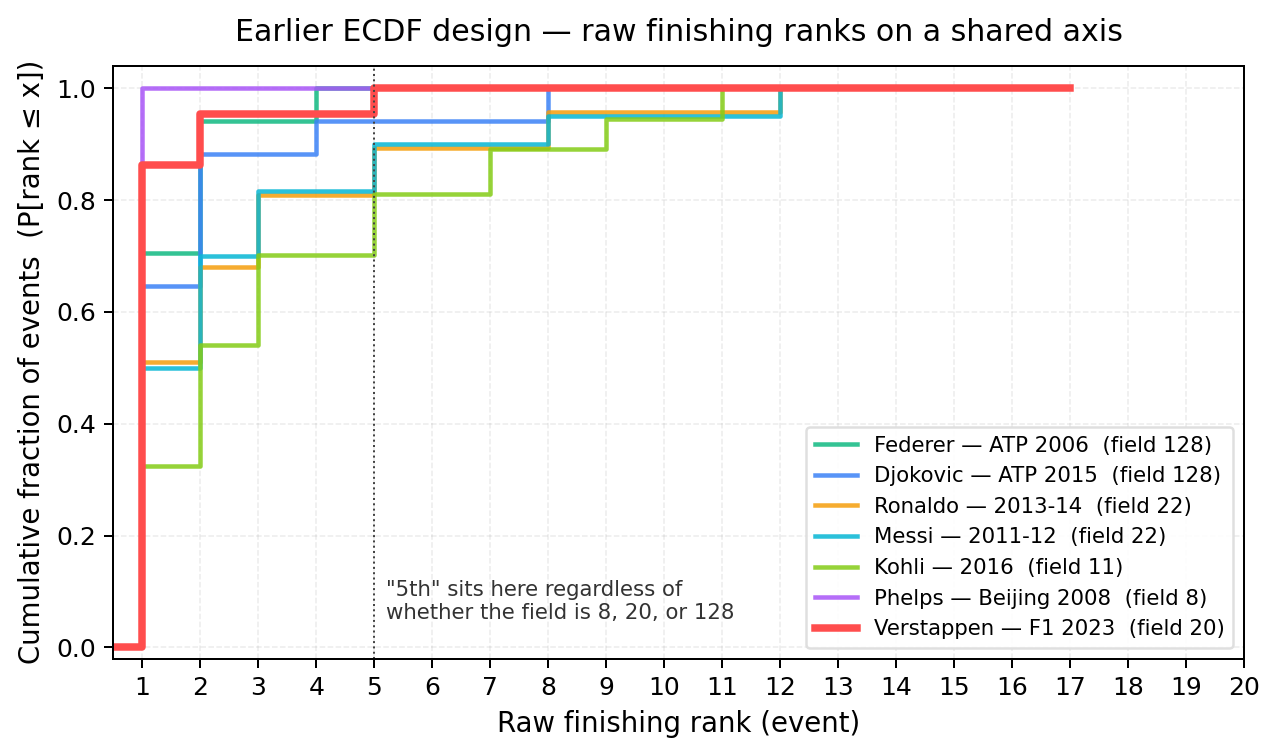
\includegraphics[width=\columnwidth]{old.png}}
\caption{Beta-stage ECDF approach using raw finishing ranks across sports. Although visually readable, the shared x-axis implies stronger comparability than the data supports because rank 5 means very different things in fields of 8, 20, or 128 competitors. This limitation motivated the final percentile-based redesign.}
\label{fig:older-ecdf}
\end{figure}

\section{Results}
\subsection{Objective 1: Within-Season Dominance}
The animated standings view shows that dominance was not merely present at the final race; it accumulated through sustained separation after the early rounds. Figure~\ref{fig:race} captures an early-to-middle-season frame where Verstappen leads but has not yet produced the final-season chasm, making the later expansion of the gap meaningful rather than inevitable.

\subsection{Objective 2: Driver Versus Car}
The teammate comparison shows that identical machinery did not produce identical outcomes. Verstappen leads P\'erez across points, wins, podiums, poles, fastest laps, and race-by-race accumulation, which supports the argument that the RB19 was a major enabling factor but not a complete explanation of the final gap (Fig.~\ref{fig:teammate}).

\subsection{Objective 3: Formula 1 History}
The normalized historical view positions 2023 among the strongest seasons ever while preserving nuance. Verstappen remains exceptional across many axes, but other seasons still exceed him on specific dimensions, preventing the visualization from collapsing history into a single unqualified ranking (Fig.~\ref{fig:history}).

\subsection{Objective 4: Cross-Sport Dominance}
The ECDF view makes cross-sport comparison possible without pretending that a race finish, a tennis tournament result, and a swimming final are the same measurement. The result is a comparison of sustained relative excellence rather than a claim that the sports themselves are directly interchangeable (Fig.~\ref{fig:ecdf}).

\begin{figure}[!t]
\centerline{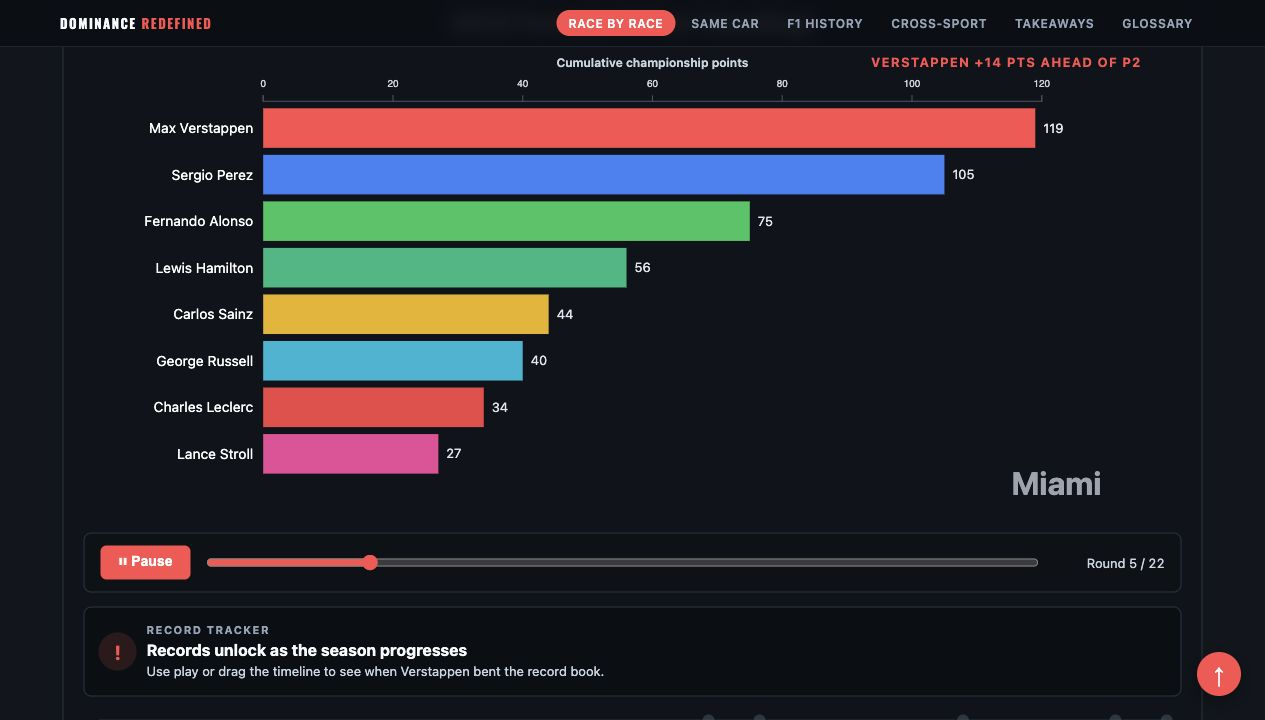
\includegraphics[width=\columnwidth]{championship.png}}
\caption{Objective 1: the bar-chart race shows cumulative standings at each round. In this frame, Verstappen already leads after Miami, while the slider and animation allow the reader to inspect how that advantage later becomes a decisive gap.}
\label{fig:race}
\end{figure}

\begin{figure}[!t]
\centerline{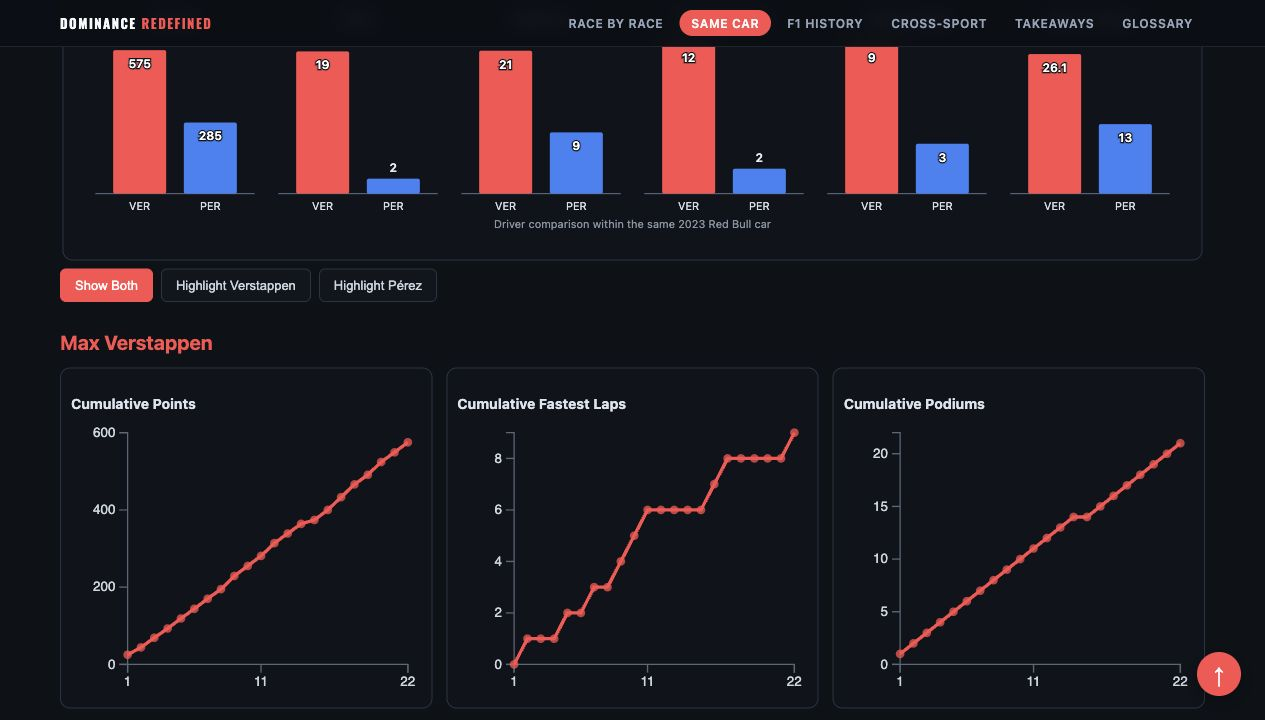
\includegraphics[width=\columnwidth]{SmallMultiples.png}}
\caption{Objective 2: season totals and the first row of small multiples compare Verstappen with P\'erez in the same RB19. The paired bars make the overall gap immediate, while the aligned time series show that the difference accumulates throughout the season.}
\label{fig:teammate}
\end{figure}

\begin{figure}[!t]
\centerline{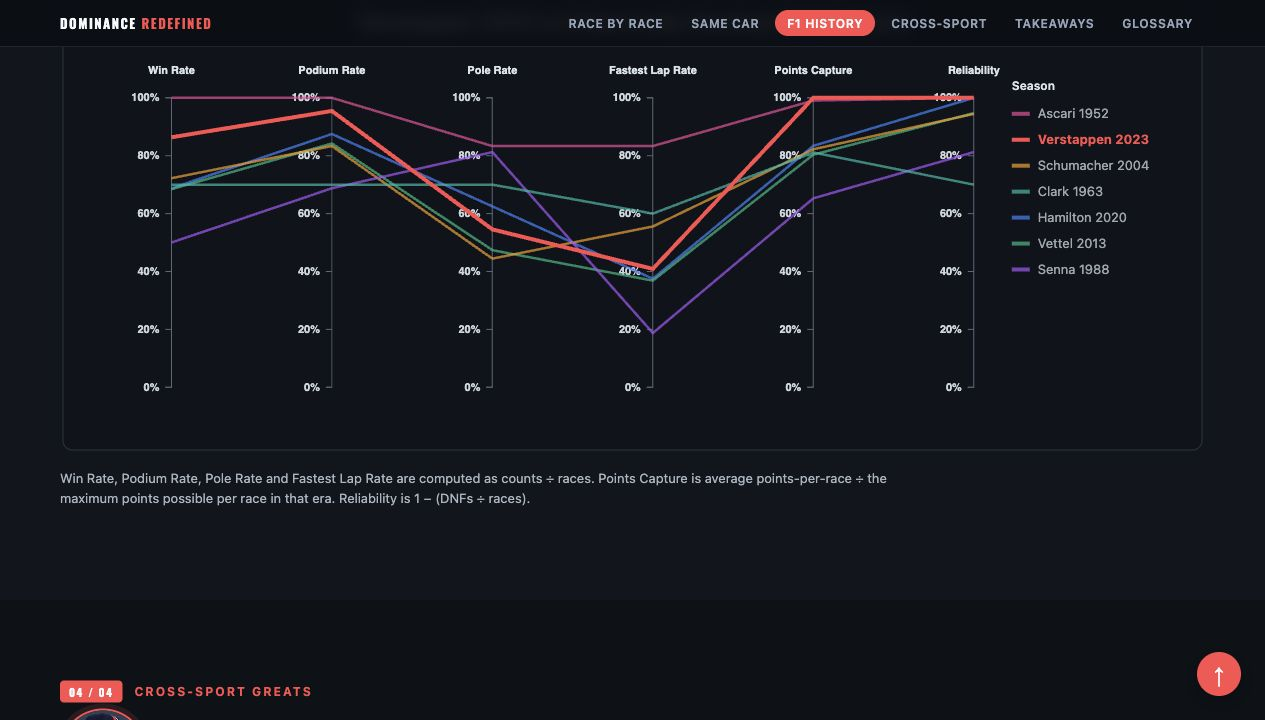
\includegraphics[width=\columnwidth]{PCP.png}}
\caption{Objective 3: normalized parallel coordinates compare historically dominant Formula 1 seasons across multiple metrics. The chart preserves nuance: Verstappen remains elite overall, while Ascari and Senna still exceed him on selected dimensions.}
\label{fig:history}
\end{figure}

\begin{figure}[!t]
\centerline{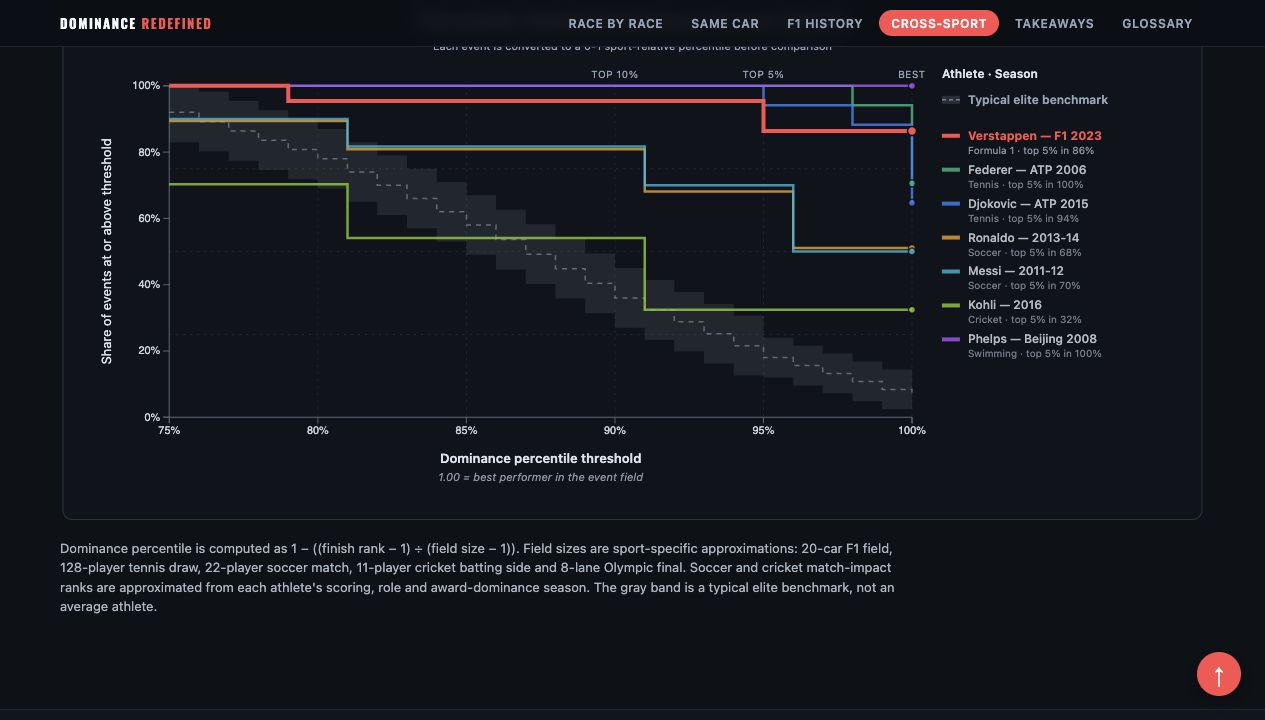
\includegraphics[width=\columnwidth]{ECDF.png}}
\caption{Objective 4: the ECDF view compares sustained relative excellence after each event is translated to a sport-relative percentile. The right side of the plot highlights how often each athlete remained near the top of their own competitive field.}
\label{fig:ecdf}
\end{figure}

\subsection{Measuring Success}
Success was measured by whether each visualization answered a distinct project objective, whether viewers could recover the intended comparison without relying on prose alone, whether interactive controls exposed additional detail without hiding the main claim, and whether the system became more honest as the analytical scope widened. The final design is successful when it communicates not simply that Verstappen was dominant, but \emph{how}, \emph{relative to whom}, and \emph{under what assumptions}.

\section{Discussion}
The overall approach is promising because it avoids forcing one chart to answer every question. The strongest design decision is the progressive widening of context: the reader first sees a familiar season story, then a controlled teammate comparison, then a historical comparison, and only afterward a cautious cross-sport abstraction. This order earns the more ambitious claims rather than presenting them as spectacle.

A stronger future variant would include explicit uncertainty or sensitivity analysis for the cross-sport percentile model, especially where soccer and cricket event ranks rely on approximations rather than naturally shared tournament structures. The project also reinforced that fairness in visualization is not one fixed rule; it depends on the question being asked and the transformations needed to make comparison meaningful.

If starting again, I would formalize the data model earlier and decide the cross-sport comparison rule sooner. The project became stronger once the design stopped asking, ``what else can be shown?'' and started asking, ``what comparison is defensible here?''.

\section{Future Work}
Future work could add linked highlighting across views, user-controlled metric weighting for the historical comparison, richer annotation of rule changes across Formula 1 eras, and a more rigorous cross-sport dataset built from event-level records rather than hand-curated approximations. A lightweight user study could also test whether readers correctly interpret the difference between raw totals, normalized rates, and percentile-based dominance.

\section{AI Use Disclosure}
Generative AI was used as a support tool during the project for wording refinement, limited CSV cleanup and name normalization, and finding possible resources for manual review. It was not treated as an authoritative data source: numeric values used in the final visualizations were checked against the underlying records before inclusion.

\section{Conclusion}
This project uses interactive visualization to turn a familiar sports claim into a sequence of testable comparisons. By moving from season progression to teammate control, historical normalization, and cross-sport percentiles, it shows that Verstappen's 2023 season was not merely record-setting but structurally dominant across multiple analytical frames. At the same time, the project argues that good visualization should sharpen claims rather than inflate them.

\bibliographystyle{IEEEtran}
\bibliography{references}

\end{document}
